\documentclass[letterpaper,12pt]{article}
\usepackage{calc,layout,epsfig,setspace,palatino,booktabs,rotating,multirow,amsmath,hyperref}
\title{Temperature and Wavelength Dependence of Refractive Index for Solid Noble Gas Films}
\author{Joseph Noonan\footnote{noonan AT frib DOT msu DOT edu}\\ Spinlab: \href{https://spinlab.me}{http://spinlab.me} \\ National Superconducting Cyclotron Laboratory\\ Michigan State University}
\date{\today}
%%%%%%%%%%%%%%%%%%%%     page layout     %%%%%%%%%%%%%%%%%%%%
%  1 pt = 1/72.27 in
%  page 99 of the LaTeX book
\pagestyle{plain}
%%%%% horizontal stuff
\oddsidemargin = 0pt
\evensidemargin = 0pt
\marginparsep = 0pt
\marginparwidth = 0pt
\textwidth = 469pt
%%%%% vertical stuff
\normalsize
\setlength{\textheight}{\baselineskip*44+\topskip}
\topmargin = 0pt
\headheight = 0pt
\headsep = 0pt
\footskip = 30pt%%%%%%%%%%%%%%%%%%%%     defs     %%%%%%%%%%%%%%%%%%%%
\newcommand{\ket}[1]{\ensuremath{\left | #1 \right > }}
\newcommand{\bra}[1]{\ensuremath{\left < #1 \right | }}
\newcommand{\braket}[2]{\ensuremath{\left < #1 \mid #2 \right > }}
\newcommand{\tensor}[1]{\ensuremath{ \stackrel{\leftrightarrow}{#1} } }
\newcommand{\munu}{\ensuremath{ {\mu\nu} }}
\newcommand{\up}{\ensuremath{\uparrow}}
\newcommand{\dn}{\ensuremath{\downarrow}}
\newcommand{\nn}{\ensuremath{\nonumber \\ }}
\newcommand{\sci}[2]{\ensuremath{#1\!\times\!10^{#2}}}
\newcommand{\degC}{\ensuremath{\,\mathrm{^\circ C}}}
\newcommand{\degK}{\ensuremath{\mathrm{K}}}
\newcommand{\tw}[1]{\noindent\bf \hphantom{*}\rm\ #1\\}
\newcommand{\ta}[1]{\noindent\bf *\rm\ #1\\}
\newcommand{\tb}[2]{\noindent\bf #1\rm\ #2\\}
\newcommand{\ts}[2]{\noindent\bf \hphantom{#1}\rm\ #2\\}
\newcommand{\iso}[2]{$^{#2}\mathrm{#1}$}
\newcommand{\jb}[5]{\item #1, #2.\ \href{#5}{\textsl{#3}.\ #4}.}
\newcommand{\tn}[3]{\item \href{#3}{#1}, #2.}
\newcommand{\cs}[3]{\item #1. #2. \textsl{#3}.}
\newcommand{\id}[3]{\item \textsl{#3}, #2. #1.}
\usepackage{graphicx}
\usepackage{subcaption}

\begin{document}

\maketitle

The paper "Refractive Indices of the Condensed Inert Gases" (Sinnock and Smith 1969) contains data for the refractive indices of solid krypton and argon films at certain temperatures and wavelengths. The data is summarized as follows:
\begin{figure}[h!]
	\begin{subfigure}[b]{0.5\linewidth}
		\centering
		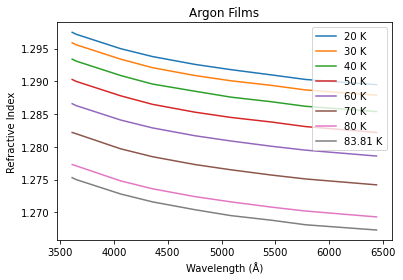
\includegraphics[width=\textwidth,height=\textheight,keepaspectratio]{argon1.png}
	\end{subfigure}
	\begin{subfigure}[b]{0.5\linewidth}
		\centering
		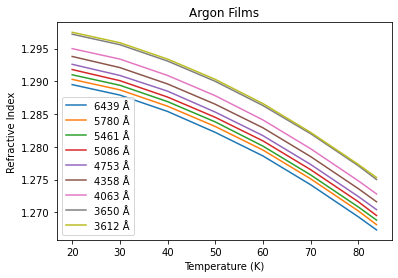
\includegraphics[width=\textwidth,height=\textheight,keepaspectratio]{argon2.png}
	\end{subfigure}
	\begin{subfigure}[b]{0.5\linewidth}
		\centering
		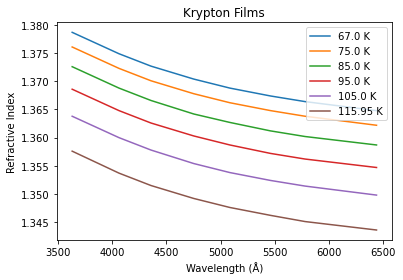
\includegraphics[width=\textwidth,height=\textheight,keepaspectratio]{krypton1.png}
	\end{subfigure}
	\begin{subfigure}[b]{0.5\linewidth}
		\centering
		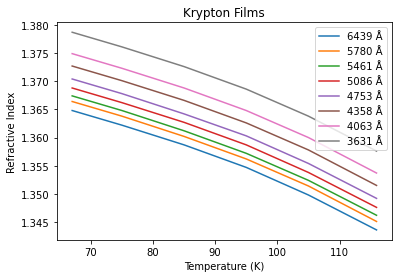
\includegraphics[width=\textwidth,height=\textheight,keepaspectratio]{krypton2.png}
	\end{subfigure}
\end{figure}

Based on a first-order approximation for thermal expansion, $l_T=(1+aT)l_0$, where $l_T$ is the length of a solid at temperature $T$ (in Kelvin), $l_0$ is the length at absolute zero, and $a$ is a constant, it was expected that $n=\sqrt{1+\alpha\rho_T}=\sqrt{1+\frac{b}{(1+aT)^3}}$, where $n$ is the refractive index, $\alpha$ is the polarizability of the material, $\rho_T$ is the number density of particles, and $b$ is another constant. However, this approximation did not fit with the data on the refractive index of noble gas films from the paper because, as seen in the graphs, the temperature-vs-refractive-index function is concave and decreasing, while the function above is always either convex and decreasing, concave and increasing, or constant, depending on the parameters. Therefore, a second-order approximation was used for thermal expansion, yielding the new formula, $$n=\sqrt{1+\frac{b}{(1+aT+cT^2)^3}}.$$
This formula gives a good fit for the temperature dependence of refractive index at any given wavelength for both krypton and argon films. The refractive index of a substance at different wavelengths can be given approximately by the formula $n_\lambda=A+\frac{B}{\lambda^2}+\frac{C}{\lambda^4}$, where $\lambda$ is the wavelength, and $A$, $B$, and $C$ are constants, according to the paper "Rayleigh, Mie, and Tyndall scatterings of polystyrene microspheres in water: Wavelength, size, and angle dependences" (He et al, 2009)). I would like to try to combine these two effects into a single formula. My first attempt to do so was to start with the temperature dependence formula and multiply by a factor proportional to $A+\frac{B}{\lambda^2}+\frac{C}{\lambda^4}$, yielding the formula $$n=\sqrt{1+\frac{b}{(1+aT+cT^2)^3}}(d+\frac{e}{\lambda^2}+\frac{f}{\lambda^4}),$$ where $d$, $e$, and $f$ are constant parameters. This formula, however, did not yield a good fit for the data. This was the best fit that could be acheived for krypton films. 
\begin{figure}[h!]
	\centering
	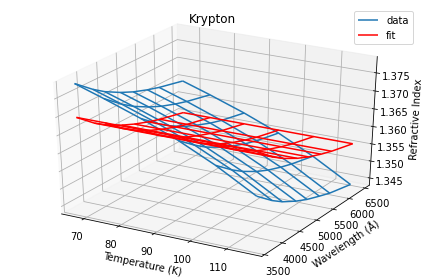
\includegraphics[width=0.5\textwidth,height=\textheight,keepaspectratio]{kryptonbad.png}
\end{figure}

To get a better fit, I looked at the differences between refractive indices of films at the same temperature but different wavelengths. What I found is that the difference in refractive index of a film at a certain temperature between two different wavelengths is essentially constant, regardless of the temperature. I also found that, when I consider this difference as a function of wavelength, it fits very well with the wavelength-dependence formula. This suggests that, insteading of multiplying the temperature-dependence formula by a wavelength dependent function, I should add the wavelength-dependent function.
\begin{figure}[h!]
	\begin{subfigure}[t]{0.5\linewidth}
		\centering
		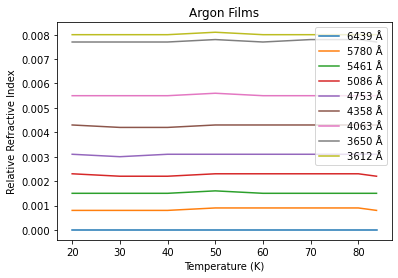
\includegraphics[width=\textwidth,height=\textheight,keepaspectratio]{argon3.png}
	\end{subfigure}
	\begin{subfigure}[t]{0.5\linewidth}
		\centering
		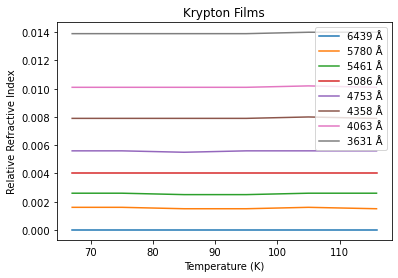
\includegraphics[width=\textwidth,height=\textheight,keepaspectratio]{krypton3.png}
	\end{subfigure}
	\caption{"Relative refractive index" means the refractive index of a film at a given temperature and wavelength, minus the refractive index of a film at the same temperature for light with a wavelength of 6439 Å.}
\end{figure}

The final formula that I used was  
\begin{equation}
n=\sqrt{1+\frac{b}{(1+aT+cT^2)^3}}+A+\frac{B}{\lambda^2}.
\end{equation}
 I removed the term $\frac{C}{\lambda^4}$ because it made no difference to the fit (The curve\_fit function in Python just left the parameter $C$ at its default value rather than varying it, suggesting that the value of $C$ was small enough that the term $\frac{C}{\lambda^4})$ was negligible). This yielded fits that were very close to the data. In fact, for both krypton and argon, the fit and the data appear right on top of each other, so the two don't even look distinct on the graph.
\begin{figure}[h!]
	\begin{subfigure}[t]{0.5\linewidth}
		\centering
		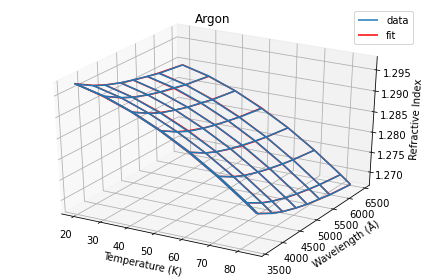
\includegraphics[width=\textwidth,height=\textheight,keepaspectratio]{argongood.png}
	\end{subfigure}
	\begin{subfigure}[t]{0.5\linewidth}
		\centering
		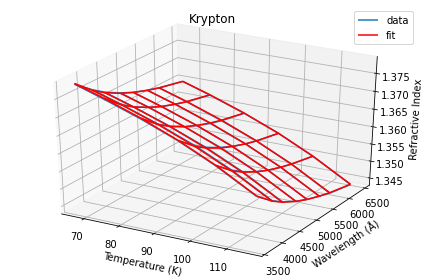
\includegraphics[width=\textwidth,height=\textheight,keepaspectratio]{kryptongood.png}
	\end{subfigure}
\end{figure}

The root mean squared errors of both the krypton and argon refractive index fits were \sci{1}{-4}. The plots of the residuals are shown below. It should be noted, however, that the original paper from which he true refractive indices are taken had the ten thousandths place as the least significant digit, so residuals smaller than \sci{1}{-4} are not actually meaningful.

\begin{figure}[h!]
	\begin{subfigure}[b]{0.5\linewidth}
		\centering
		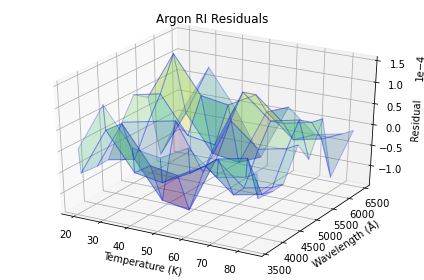
\includegraphics[width=\textwidth,height=\textheight,keepaspectratio]{argonres1.png}
	\end{subfigure}
	\begin{subfigure}[b]{0.5\linewidth}
		\centering
		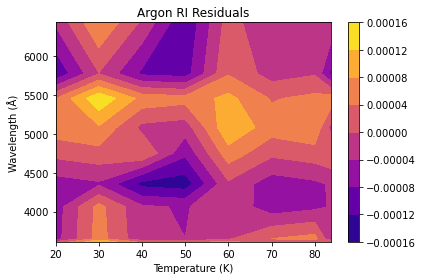
\includegraphics[width=\textwidth,height=\textheight,keepaspectratio]{argonres2.png}
	\end{subfigure}
	\begin{subfigure}[b]{0.5\linewidth}
		\centering
		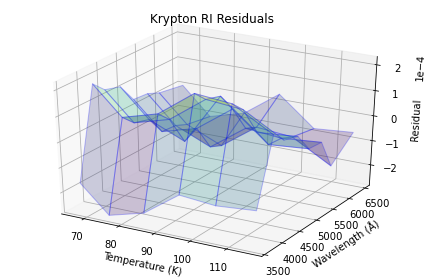
\includegraphics[width=\textwidth,height=\textheight,keepaspectratio]{krypres1.png}
	\end{subfigure}
	\begin{subfigure}[b]{0.5\linewidth}
		\centering
		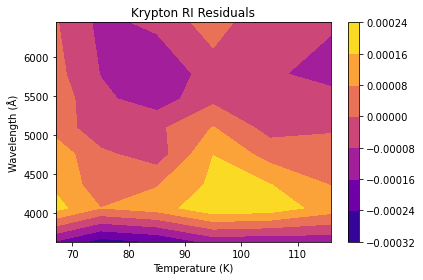
\includegraphics[width=\textwidth,height=\textheight,keepaspectratio]{krypres2.png}
	\end{subfigure}
	\caption{Both 3D and 2D plots of the residuals are given, since it is diffucilt to see all the data on the 3D plots.}
\end{figure}

Strangely, the values of the best fit parameters were not values that were expected based on what those parameters theoretically represent, especially for the krypton films. The $a$, $b$, and $c$ parameters were expected to be positive, but they were all negative for the krypton films. However, despite this, they still give a very good empirical fit.

\begin{table}[h!]
\begin{tabular}{|l|r|r|r|r|r|} \hline
Film Type & $a$ & $b$ & $c$ & $A$ & $B$      \\ \hline 
Argon&	\sci{-1.2917}{-5}&      \sci{6.3077}{-1}&        \sci{4.9294}{-6}&   \sci{1.0126}{-2}&   \sci{1.5160}{5}	 \\ \hline
Krypton&	\sci{-2.0282}{-3}&	\sci{-4.2071}{-2}&        \sci{-2.6149}{-6}&   \sci{3.9280}{-1}&   \sci{2.7206}{5}         \\ \hline	
\end{tabular}
\caption{The best fit parameters for Equation (1)}
\end{table}

Using the model from Equation (1) and the best fit parameters, the refractive indices of argon and krypton films were estimated for a range of temperatures and wavelengths that includes the temperatures of the films and the range of wavelengths used in the transmission experiments.

\begin{figure}[h!]
	\begin{subfigure}[t]{\linewidth}
		\centering
		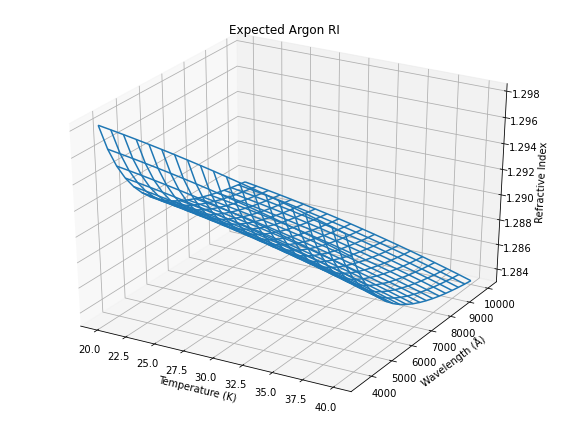
\includegraphics[width=\textwidth,height=\textheight,keepaspectratio]{arex.png}
	\end{subfigure}
	\begin{subfigure}[t]{\linewidth}
		\centering
		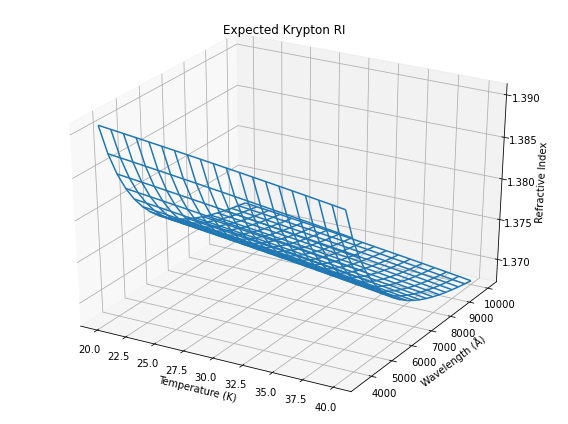
\includegraphics[width=\textwidth,height=\textheight,keepaspectratio]{krex.png}
	\end{subfigure}
\end{figure}

\end{document}



































